\section{Numerical Examples}
\vspace*{-0.2cm}
All the numerical experiments in this section are run for models of size 3 km $\times$ 2 km in the X and Z directions respectively, with a 5 m $\times$ 5 m grid spacing. Sources are placed every 50 m on the surface. The inversion is performed over the frequency band $6.67 \; \text{Hz} \leq \omega / 2 \pi \leq 30 \; \text{Hz}$, which is uniformly divided into $N_\omega = 50$ discrete frequencies. We use a Gaussian spectrum for the source wavelet (in the frequency domain), centered at 18 Hz with a standard deviation of 7 Hz. In addition we apply a linear taper (decaying to zero) on either side of the spectrum between 6.67 - 9 Hz, and 27.67 - 30 Hz. The TFWI linear inverse problem is solved in each case using the method outlined in \cite{Sarkar.sep.172.rahul1}, and for simplicity we set $\gamma = 0$ in all the tests.

\vspace*{-0.4cm}
\begin{figure}[h]
\centering
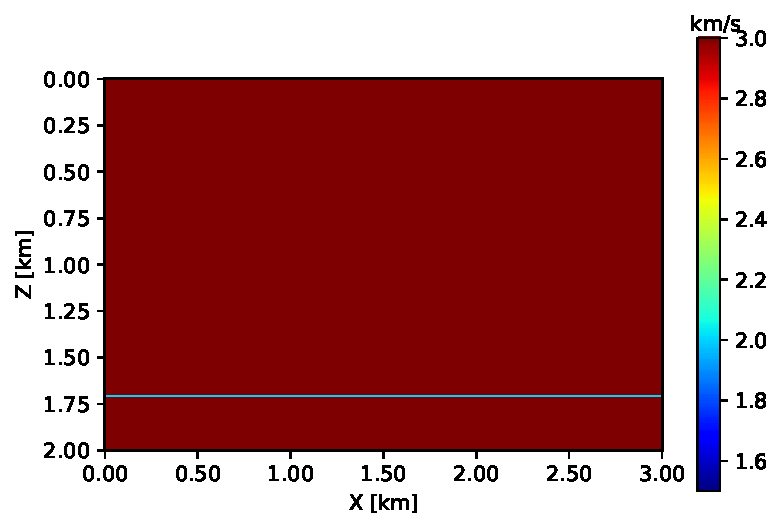
\includegraphics[width=0.8\linewidth]{Fig/veltrue-noanomaly.pdf}

\vspace*{-0.4cm}
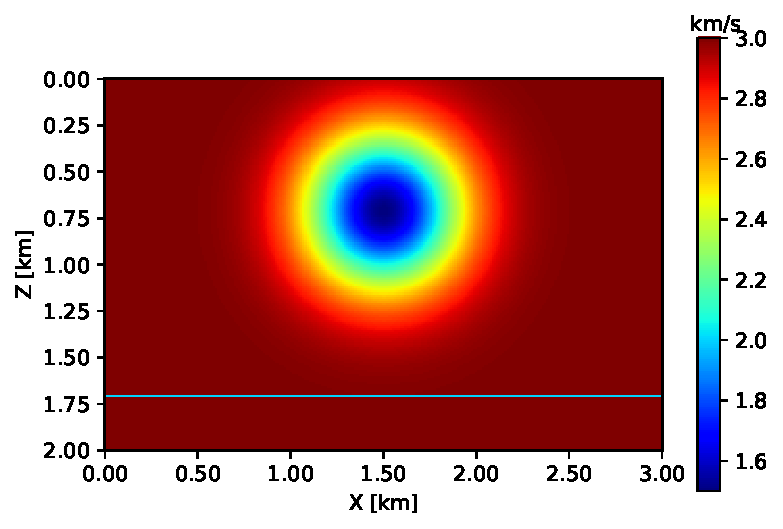
\includegraphics[width=0.8\linewidth]{Fig/veltrue-anomaly.pdf}

\vspace*{-0.5cm}
\caption{Background models without (top) and with low velocity Gaussian anomaly (bottom). The reflector is overlain at a depth of 1.71 km.}
\label{fig:example1_models}
\end{figure}

\subsection{Illumination compensation for a low velocity anomaly}

\vspace*{-0.1cm}
In the first example, we consider two cases corresponding to the models shown in Figure \ref{fig:example1_models}, one of which contains a low velocity Gaussian anomaly, and the other one has a constant velocity of 3 km/s. The reflector is placed in both cases at a depth of 1.71 km (which is overlain on the figure), and used to generate the Born data $\residh_{ki}$ with a split spread acquisition geometry, and maximum offset of 2 km. The displayed models (without the displayed reflector) form the background velocities for the linear inversion. 

\vspace*{-0.3cm}
\begin{figure}[h]
\centering
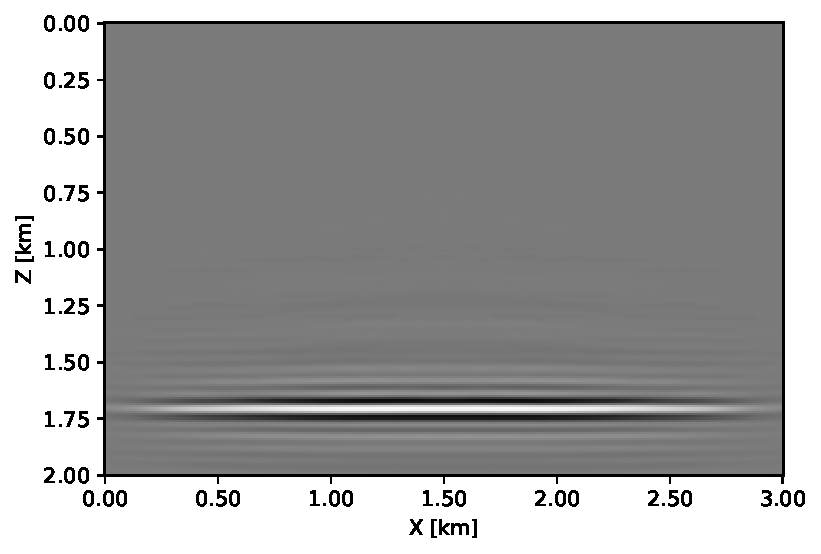
\includegraphics[width=0.7\linewidth]{Fig/noanomaly-inverted-image-stack.pdf}

\vspace*{-0.3cm}
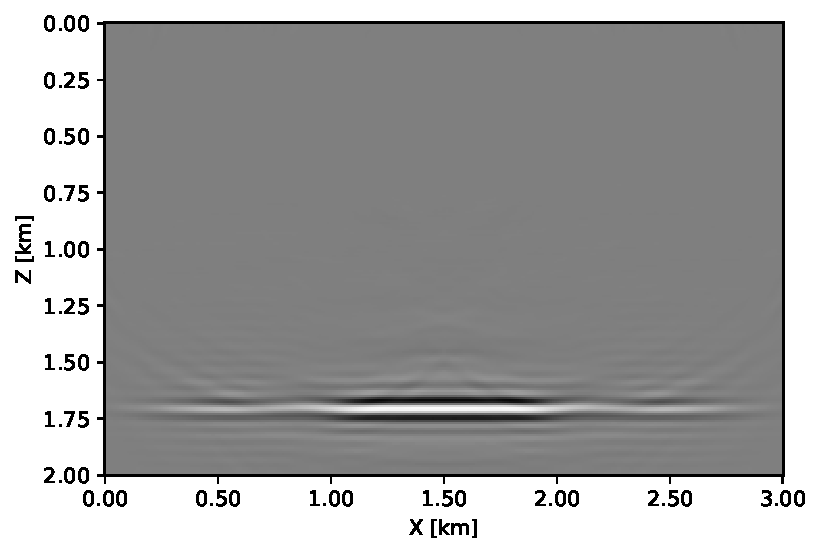
\includegraphics[width=0.7\linewidth]{Fig/anomaly-inverted-image-stack.pdf}

\vspace*{-0.5cm}
\caption{Stacked inverted images $\dmorig^{\ast}$ without regularization ($\epsilon = 0$) for the constant velocity model (top), and the low velocity Gaussian anomaly model (bottom).}
\label{fig:example1_stacks_noreg}
\end{figure}
\vspace*{-0.3cm}
\begin{figure}[h]
\centering
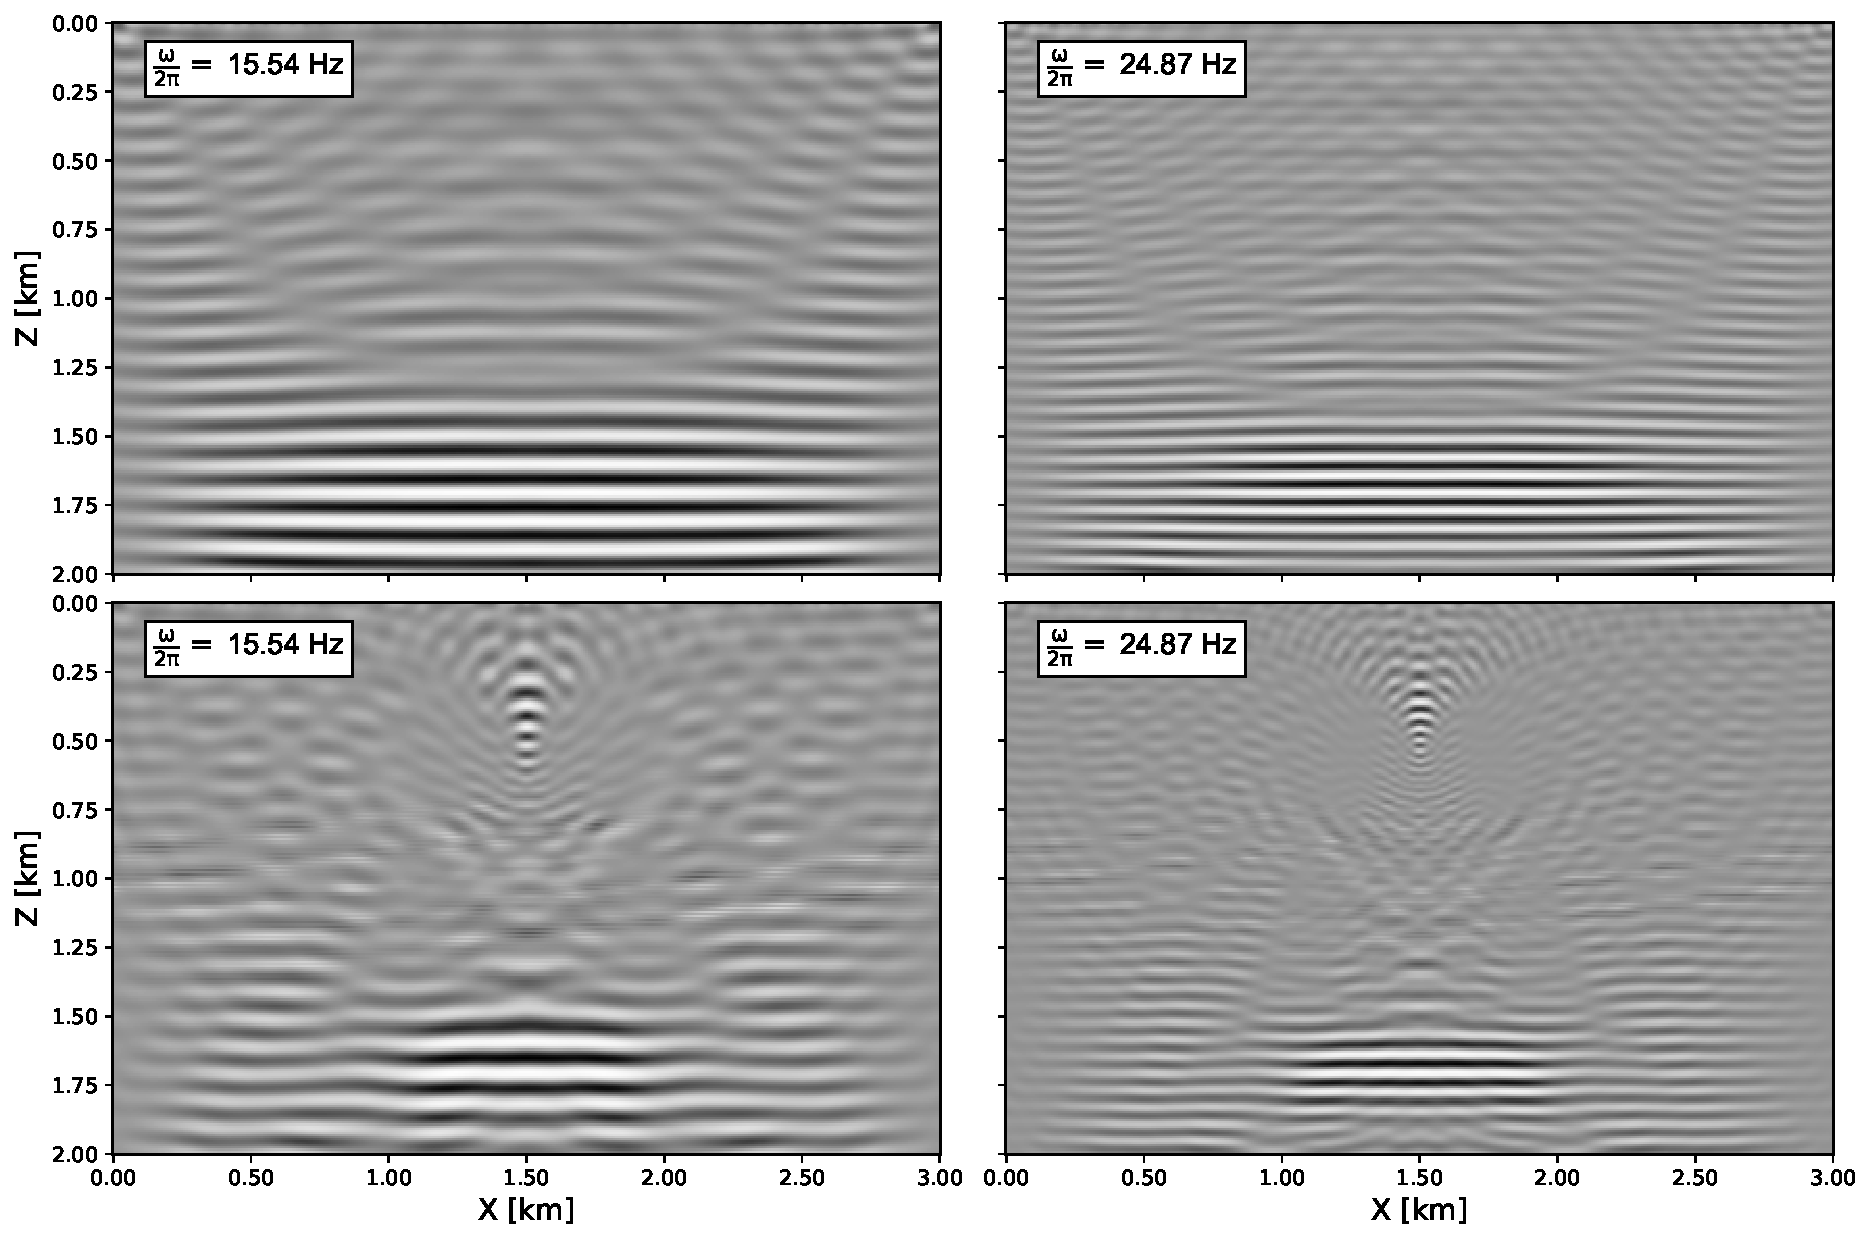
\includegraphics[width=\linewidth]{Fig/inverted-images-noreg-comparison.pdf}

\vspace*{-0.4cm}
\caption{Real parts of the inverted images $\cexth^{\ast}_k$ without regularization ($\epsilon = 0$) for the constant velocity model (top row), and the low velocity Gaussian anomaly model (bottom row). The columns correspond to $k = 20,\; \omega / 2 \pi = 15.54$ Hz (left), and $k = 40,\; \omega / 2 \pi = 24.86$ Hz (right).}
\label{fig:example1_noreg_comp}
\end{figure}

\vspace*{-0.3cm}
We first solve the linear inverse problem in both cases without any regularization ($\epsilon = 0$). The stacked inverted images for the two cases are shown in Figure \ref{fig:example1_stacks_noreg}, and the inverted images $\cexth_{k}^{\ast}$ for $k=20$ and $k=40$, corresponding to the frequencies of 15.54 Hz and 24.87 Hz respectively, are shown in Figure \ref{fig:example1_noreg_comp}. In Figure \ref{fig:example1_noreg_comp}, we have only displayed the real parts of $\cexth_{k}^{\ast}$ due to space constraints, but the imaginary parts also have similar behavior. It is clear from these illustrations that the inverted images for the Gaussian anomaly have shadow zones at some offset from the center of the model on either side, and this effect gets more prominent at larger frequencies. In fact at the reflector level, the amplitudes decrease and then increase again as one moves either to the right or to the left from the center, an effect that is most easily seen in the stacked inverted image (Figure \ref{fig:example1_stacks_noreg}). The images corresponding to the constant velocity case do not exhibit these effects, and hence we can conclude that the complexity of the background model alone causes the uneven illumination at the reflector level for the low velocity Gaussian anomaly model.

\vspace*{-0.1cm}
\begin{figure}[h]
\centering
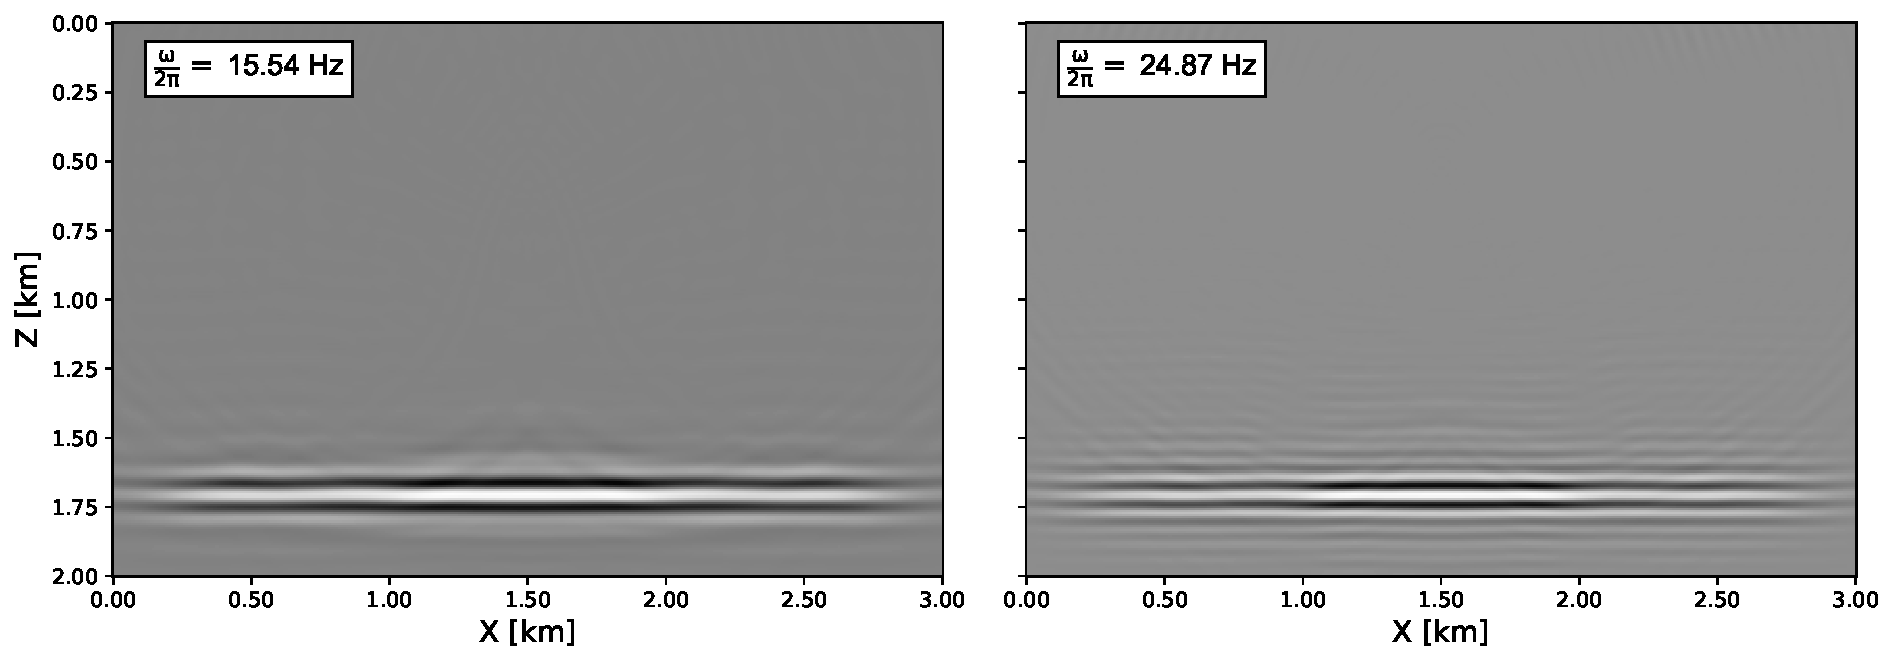
\includegraphics[width=\linewidth]{Fig/inverted-images-reg-anomaly.pdf}

\vspace*{-0.5cm}
\caption{Real parts of the inverted images $\cexth^{\ast}_k$ with regularization ($\epsilon = 0.2$) for the low velocity Gaussian anomaly model. The images correspond to $k = 20,\; \omega / 2 \pi = 15.54$ Hz (left), and $k = 40,\; \omega / 2 \pi = 24.86$ Hz (right).}
\label{fig:example1_images_reg}
\end{figure}

\vspace*{-0.2cm}
\begin{figure}[h]
\centering
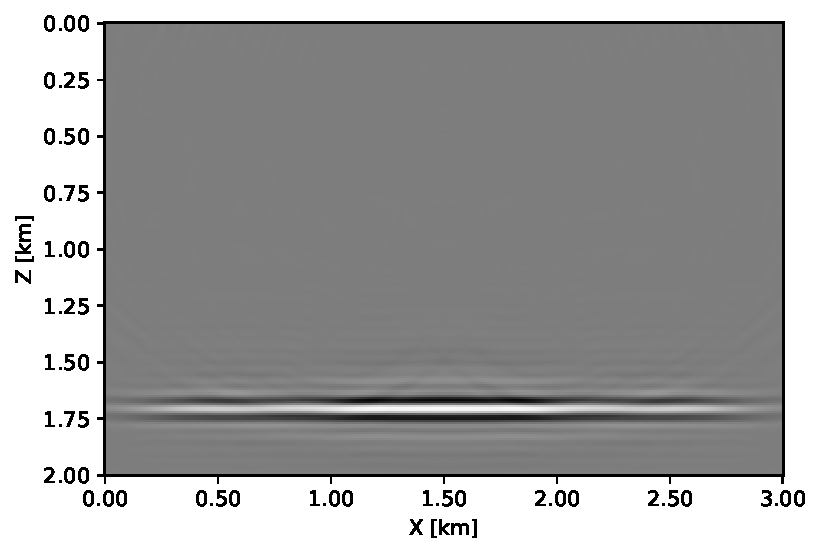
\includegraphics[width=0.7\linewidth]{Fig/anomaly-inverted-image-stack-reg.pdf}

\vspace*{-0.5cm}
\caption{Stacked inverted image $\dmorig^{\ast}$ with regularization  for the low velocity Gaussian anomaly model ($\epsilon = 0.2$).}
\label{fig:example1_stack_reg}
\end{figure}

\vspace*{-0.2cm}
We now show what happens when we turn on the regularization in the linear inversion, where after some tests the regularization strength was set at $\epsilon = 0.2$. In Figure \ref{fig:example1_stack_reg} we have displayed the stacked inverted image with the Gaussian anomaly model, while in Figure \ref{fig:example1_images_reg} the inverted images are shown at the same two frequencies as in Figure \ref{fig:example1_noreg_comp} to enable a direct comparison. We see that the effect of regularization is to ``equalize'' the inverted images, which is clearly seen in Figure \ref{fig:example1_images_reg} as the images tend to become similar to each other across frequencies. This is to be contrasted with the bottom-row images in Figure \ref{fig:example1_noreg_comp} where there is great variation between the images at the two frequencies with the same Gaussian anomaly model. The net effect of this phenomenon on the stacked inverted image in Figure \ref{fig:example1_stack_reg} is that in comparison to the bottom image in Figure \ref{fig:example1_stacks_noreg}, the reflector has been imaged more uniformly and continuously.

\subsection{Illumination compensation for a low velocity anomaly and acquisition hole}

\vspace*{-0.1cm}
In the second example we take exactly the same low velocity Gaussian anomaly model, the same reflector configuration, and the same acquisition configuration, except that all sources and receivers have been removed in a 0.5 km region, centered over the location of the Gaussian anomaly. In physical coordinates, this corresponds to the region $X = 1.25 - 1.75$ km. We again perform the same experiments --- solve the TFWI linear inverse problem with and without regularization. The value $\epsilon=0.2$ was chosen for the regularized inversion. The stacked inverted images for the two cases are displayed in Figure \ref{fig:example2_images_stacks}, while the inverted images are shown for the same two frequencies (as in the first example) for these cases in Figure \ref{fig:example2_image_comp}. Just like the first example, it is observed that the effect of the regularization term is to equalize the inverted images over frequencies, that leads to better continuity and illumination compensation of the reflector in the stacked inverted image.

\vspace*{-0.2cm}
\begin{figure}[h]
\centering
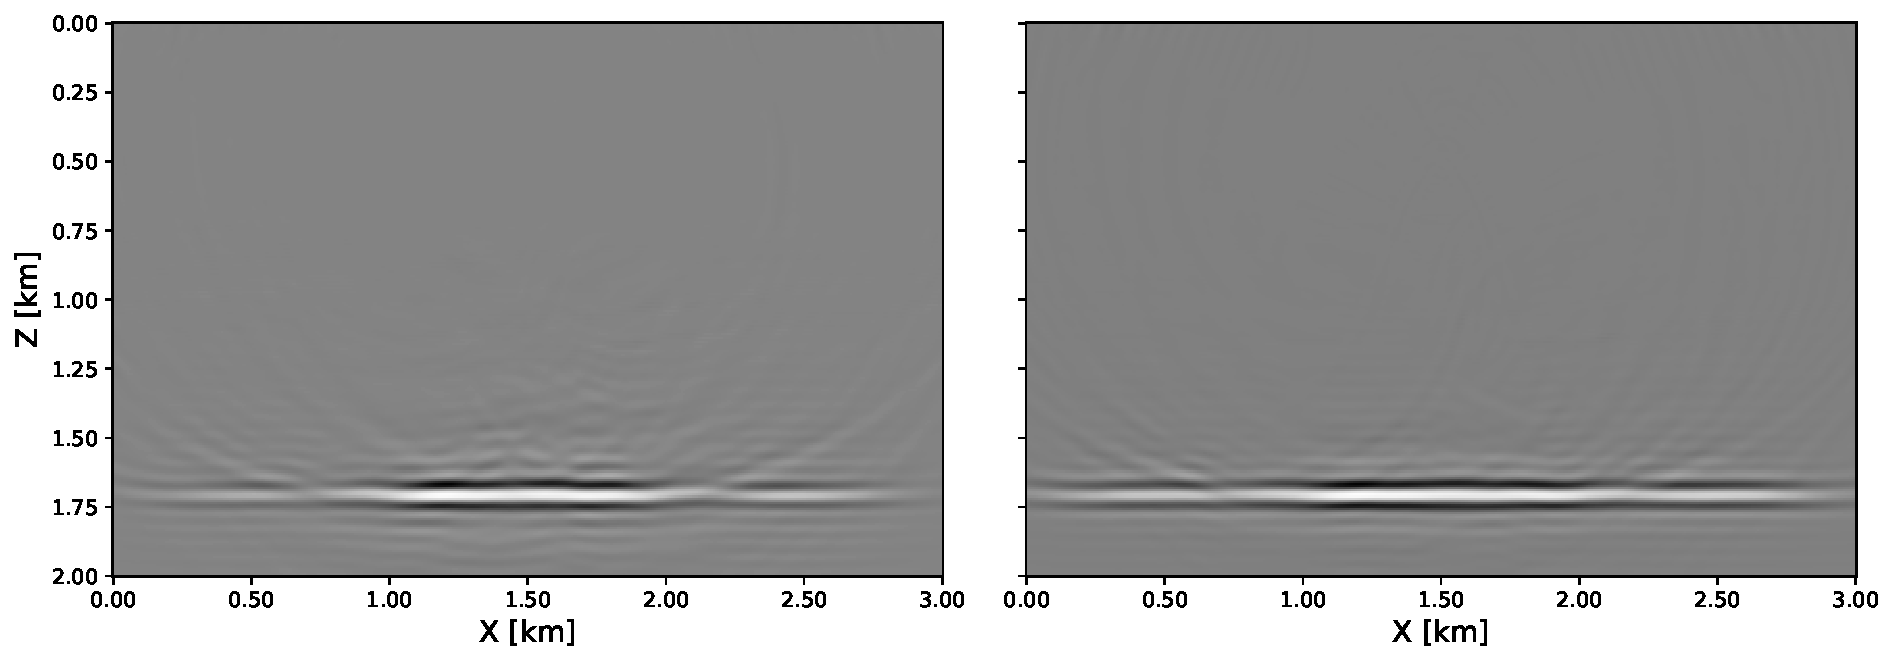
\includegraphics[width=\linewidth]{Fig/anomaly-hole-inverted-image-stack-comp.pdf}

\vspace*{-0.5cm}
\caption{Stacked inverted images $\dmorig^{\ast}$ with regularization (right), and without regularization (left) for the low velocity Gaussian anomaly model, in the presence of acquisition hole.}
\label{fig:example2_images_stacks}
\end{figure}
\vspace*{-0.2cm}
\begin{figure}[h]
\centering
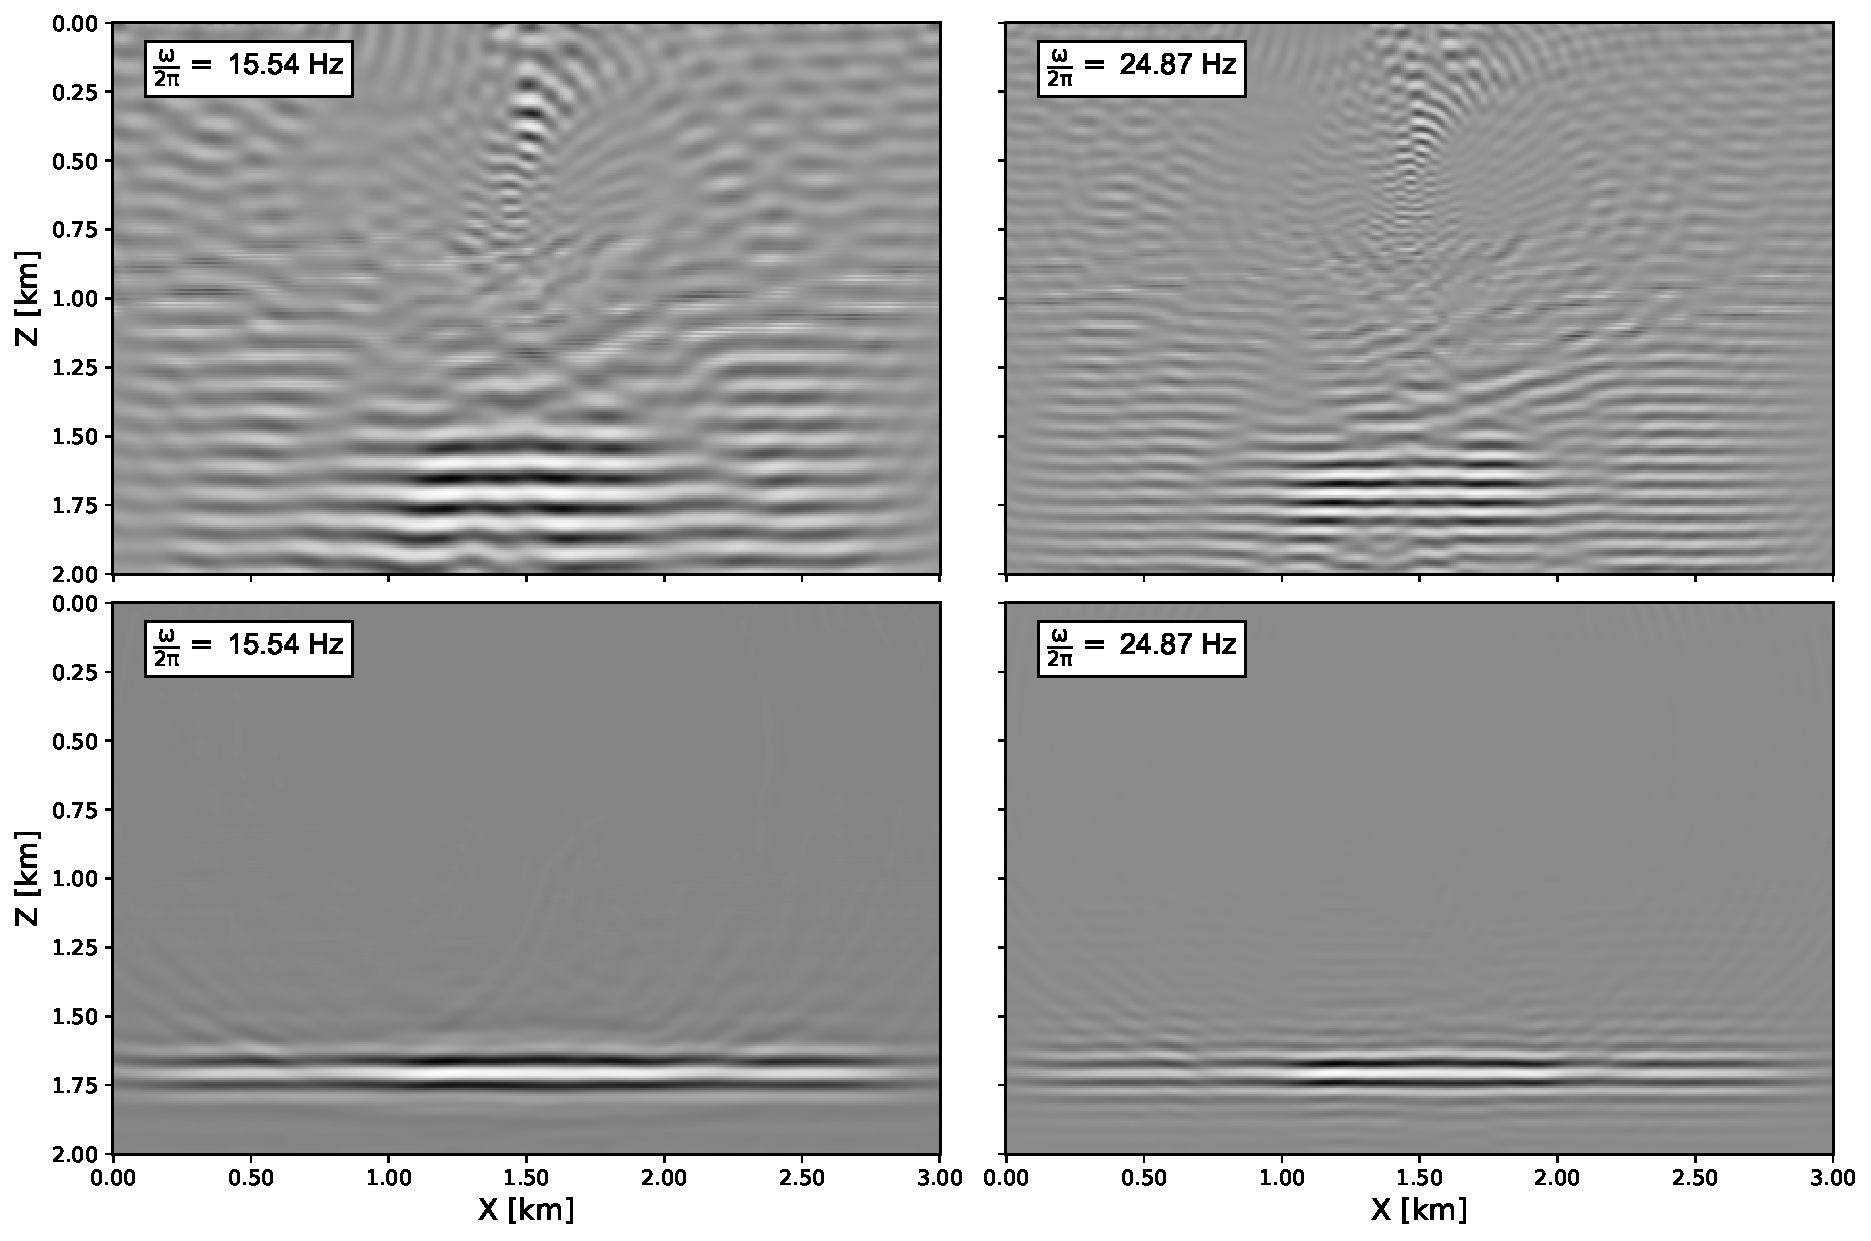
\includegraphics[width=\linewidth]{Fig/hole-inverted-images-comparison.pdf}

\vspace*{-0.4cm}
\caption{Real parts of the inverted images $\cexth^{\ast}_k$ in the presence of acquisition hole for the low velocity Gaussian anomaly model. The rows correspond to the cases without regularization (top), and with regularization (bottom). The columns correspond to $k = 20,\; \omega / 2 \pi = 15.54$ Hz (left), and $k = 40,\; \omega / 2 \pi = 24.86$ Hz (right).}
\label{fig:example2_image_comp}
\end{figure}